%# -*- coding: utf-8 -*-
% !TEX encoding = UTF-8 Unicode
\RequirePackage{fixltx2e}
\documentclass[aps,pre,12pt,preprint,onecolumn,showpacs,showkeys,UTF8]{revtex4-1}
\usepackage{ctex}
\usepackage{setspace,dcolumn}
\usepackage{subfig}
\usepackage{graphicx,psfrag,epsfig}
\usepackage[font=small,format=plain,labelfont=bf,textfont=it,justification=raggedright,singlelinecheck=false]{caption}
\usepackage{amsmath,amsfonts,amssymb,amsthm,bm,upgreek}
\usepackage{geometry}
\usepackage[mathscr]{eucal}
\usepackage{titlesec}
\titleformat{\section}{\bf\fangsong\zihao{4}}{\thesection}{0.75em}{}
\geometry{top=2.54cm,bottom=2.54cm,left=3cm,right=3cm}
\renewcommand\appendixname{附录}
\renewcommand\abstractname{}%摘要
\renewcommand\tablename{表}
\renewcommand\figurename{图}
\makeatletter
\def\@keys@name{\songti\zihao{-4}{\bf 关键词:}}
\def\Received@name{\zihao{-5}{接收} }
\def\Revised@name{\zihao{-5}{修订} }
\def\Accepted@name{\zihao{-5}{采纳} }
\def\Published@name{\zihao{-4}{发表} }
\makeatother
\linespread{1.6}
\renewcommand{\labelenumi}{\alph{enumi}.}
\leftmargini=20mm

\begin{document}

\title{\bf\heiti\zihao{3}电子自旋共振\vspace{15mm}}
\author{\fangsong 乔颢\vspace{2mm}}
\affiliation{\songti\zihao{-4}北京大学物理学院2011级2班~~~~学号:1100011354 \vspace{2mm}}
\keywords{电子自旋共振,微波,共振吸收}
\email{1993422qsh@gmail.com; 18600200672}
\begin{abstract}
	\vspace{10mm}
	\begin{spacing}{1.5}
		\songti\zihao{-4}
		此部分为摘要. 200―300字,说明用什么方法做了什么事,由此得到什么结果和结论,有何意义. 摘要中不用缩略词,不用第一人称.
	\end{spacing}
\end{abstract}

\maketitle

\section{引言}
电子自旋共振(ESR)或者说电子顺磁共振(EPR)是指在含有未成对电子的原子、离子或者分子的顺磁性物质,在稳恒磁场的作用下原始能级劈裂,对合适的微波能量发生的能级间的共振跃迁吸收现象。如果共振仅仅涉及物质中的电子则被称为电子的自旋共振,而在一般情况下,电子的轨道磁矩不可忽略,所以被称作电子的顺磁共振。

电子顺磁共振通过观测研究对象的共振波谱,可以了解这些物质中未成对电子的电子状态以及其周围环境方面的信息。同时由于这种方法并不改变或者破坏研究对象本身的性质,因而对于那些寿命短,化学性质不稳定的分子或者自由基等的研究有着显著的作用。所以自1945年发现这个现象以来,顺磁共振已经在物理学,化学等领域中取得了广泛的应用。

这个实验目的是利用微波系统和一系列的微波器件对DPPH自由基的电子自旋共振进行观测和测量,并与理论给出的数值进行验证。从实验的结果来看,实验数据基本上支持了理论给出的预测结果。

\section{实验}
\subsection{实验原理}
按照经典的理论,原子中的电子既有轨道运动,又有自旋运动。对于单电子院子,电子轨道角动量和自旋角动量合成为电子的总角动量。有电子的总磁矩也满足:
\begin{equation}
	\bm{\mu_j}=-g_j\frac{e}{2m_e}\bm{P_j}
\end{equation}
式中$\bm{P_j}$为电子总角动量,$e$为电子电荷,$m_e$为电子质量,$g_j$则为朗德因子。其数值满足以下关系:
\begin{equation}
	\mu_j=-g_j\frac{e}{2m_e}P_j	
\end{equation}
其中:
$$P_j=\sqrt{j(j+1)}\hbar$$
朗德因子满足以下式子:
$$g_j=1+\frac{j(j+1)-l(l+1)+s(s+1)}{2j(j+1)}$$
对于研究对象DPPH(二苯基——苦基肼基)而言,他的一个氮原子上只有一个未成对电子,所以其g因子应该非常接近于自由电子的g值。

在外加磁场中的磁矩的作用能为$E=-\bm{\mu}\cdot\bm{H}$所以对于电子自旋有其磁量子数只能取两个数值,即$M_z=\pm\frac{1}{2}$所以原来的能级在外加磁场后会劈裂成两个能级,能级差与外界恒磁场成正比:
\begin{equation}
	\Delta E=E_a-E_b=g\mu_B H
\end{equation}

如果在单电子原子或者自由基分子所处的稳恒磁场区域加上一个微波场,当一个微波量子的能量正好等于上述的能级差的时候,电子在两个能级之间发生共振跃迁。所以当对磁场强度或者微波频率进行调节可以测量得到样品的g值。在本实验中改变的是磁场的强度。

\newpage
\subsection{实验装置}
实验装置如图所示:
\begin{figure}[h]
	\begin{center}
		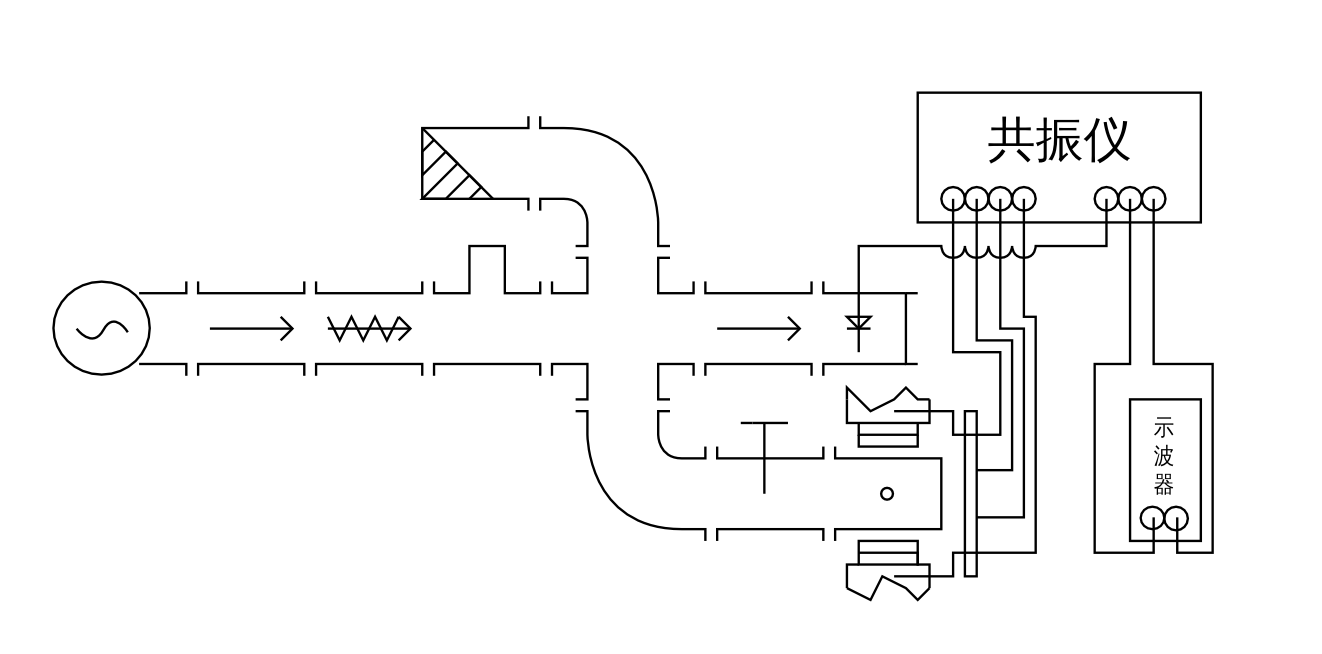
\includegraphics[width=0.8\textwidth]{pic1.png}
		\caption{\label{fig:exp1}利用微波仪器测量DPPH的朗德因子及弛豫时间的实验装置示意图}
	\end{center}
\end{figure}
其中实验装置最左端是一个产生微波的固态信号源,稳定的产生固定频率(8330MHz)的TE10电磁波,微波信号由信号源的体效应振荡器产生并可以调整其频率。微波在TE10波导管中传播,经过隔离器,衰减器,波长计进入双T接头(魔T)的H端。其中隔离器的作用是为了防止后端设备对固态源的影响,而波长计则是准确的测量管中微波的波长。在不进行波长测量的时候应该对波长计进行失谐处理而避免其影响整个微波回路。

微波信号经过魔T分别进入图示中上端和下端的负载。在合理的调节两个负载的阻抗并使之匹配之后,微波在桥路中平衡形成驻波。由麦克斯韦方程组结合魔T的边界条件可知,这时候微波不会向魔T的E端传播,所以此时E端的检波晶体就不会检测到微波信号。

魔T两侧的两臂上的一端中放有样品。未加外界磁场的时候调节调配器使得魔T平衡,而当加入合适的磁场时候,样品吸收微波形成共振,这时候改变了样品所在臂的阻抗,从而阻抗不再匹配。这样的话就可以通过检波晶体观测到顺磁共振的现象了。

\subsection
















\begin{thebibliography}{}
	\bibitem{Book} 吴思成,王祖铨~2010 近代物理实验(第三版)(北京:高等教育出版社)第xxx页.
%
	\bibitem{kw1} Chu S, Hollberg L, Bjorkholm J E, Cable A, Ashkin A 1985 {\it Phys. Rev. Lett.} {\bf 55} 48.%英文期刊
	\bibitem{kw2} 耿涛,闫树斌,王彦华,杨海菁,张天才,王军民~2005 物理学报~{\bf 54} 5104.%中文期刊
	\bibitem{kw3} 王彦华~2007 博士学位论文(太原:山西大学).%学位论文
	\bibitem{kw4} 冯端,金国钧~2003 凝聚态物理学(上卷)(北京:高等教育出版社) 第341页.%专著
	\bibitem{kw5} Tabbal A M, Mérel P, Chaker M 1999 Proceedings of the 14th International Symposium on Plasma Chemistry Prague, Czech Republic, August 2-6,1999 p1099.%会议文集
	\bibitem{kw6} Plank C J U.S. Patent 4 081 490 [1978-02-15].%专利
	\bibitem{kw7} 史寒朵~北京大学2012年近代物理实验报告:He-Ne 激光器放电性质研究. %同学实验报告
%
\end{thebibliography}

\clearpage
\appendix
\section{思考题}

\end{document} 
